%%%%%%%%%%%%%%%%%%%%%%%%%%%%%%%%%%%
\section{Case Study and Tool Support}
\label{sect:caseStudyToolSupport} %
%%%%%%%%%%%%%%%%%%%%%%%%%%%%%%%%%%%%

%This section first presents a relatively complex case, order management domain~(OrderMan), that is adapted from the OMG/UML specification~\cite[p.~396]{omg_unified_2017}. The aim is to illustrate the usability of \agl~and to investigate how our proposed method is applied to develop software for a real-world problem domain. This section then presents tool support, with a focus on explaining the main design choices and used technologies.
This section introduces a complex case study, the order management domain (\orderman), which is adapted from the OMG/UML specification~\cite[p.~396]{omg_unified_2017}. The purpose is to demonstrate the practical application of \agl and investigate how our proposed method can be used to develop software for real-world problem domains. Additionally, this section presents the tool support used, focusing on explaining the primary design choices and technologies utilized.

\begin{figure*}[ht]
	\centering
	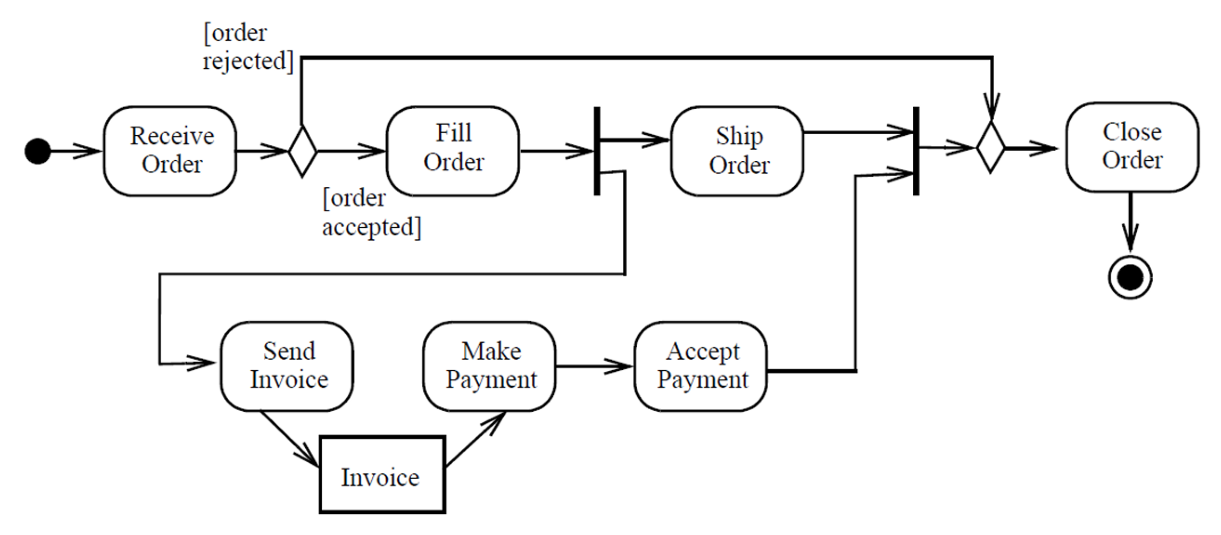
\includegraphics[scale=0.53]{orderMan_actDiagram}
	\caption{The UML activity diagram for the process to handle orders, adapted from~\cite[p.~369]{omg_unified_2017}.} %
	\vspace{-0.2cm}
	\label{fig:orderMan_actDiagram}
\end{figure*}

%%%%%%%%%%%%%%%%%%%%%%%%%%%%%%%%%%%
\subsection{Case Study: \orderman}
\label{subsect:caseStudy} %
%%%%%%%%%%%%%%%%%%%%%%%%%%%%%%%%%%%%

%Figure~\ref{fig:orderMan_actDiagram} shows the UML activity diagram for the process in \orderman to handle orders. To obtain the unified domain model for \orderman, as shown in Figure~\ref{fig:orderMan_unifiedModel}, we have applied 
%all the domain behavior patterns of our first catalog. Specifically, Figure~\ref{fig:orderMan_unifiedModel}(A) represents an activity graph with nodes labeled with numbers for the activity HandleOrder. It also represents part of the unified class model (for a full version, we refer the reader to the technical report~\cite{dang2023aglTechReport}), that consists of one activity class (\clazz{HandleOrder}), four main data classes (\clazz{CustOrder}, \clazz{Invoice}, \clazz{Shipment}, \clazz{Payment}), four control classes (\clazz{AcceptOrNot}, \clazz{Delivery}, \clazz{CompleteOrder}, \clazz{EndOrder}), and four remaining classes \wrt coordinator nodes (\clazz{FillOrder}, \clazz{CollectPayment}, \clazz{ShipOrder}, \clazz{AcceptPayment}). As explained in Section~\ref{sect:agl}, coordinator nodes are used to provide a whole picture of a task group. %
%%The coordinator's UI serves as the container of those of the member tasks, so that user can have a whole picture of the group. The member tasks themselves interact with each other to perform the group's logic.
%For example, the coordinator node Fill Order (node 3) handles the following two tasks: Update Order~(node 5) and Delivery Order~(node 6). %
%%Update Order basically updates the Order status to "Fulfilled" after the order has actually been fulfilled by the warehouse. Once this has been done, Order Delivery is performed to deliver the ordered products to the customer and to collect payment. In the above use case, %
%Fill Order simply coordinates the tasks, ensuring that Update Order is performed first then Delivery Order. It does not contribute any data to this flow. However, it enables the user to observe and perform the task flow on the UI.
Figure~\ref{fig:orderMan_actDiagram} illustrates the UML Activity diagram that depicts the process of handling orders in \orderman and Figure~\ref{fig:domain-model-orderman} show the domain model of \orderman.
\begin{figure*}[!ht]
	\centering
	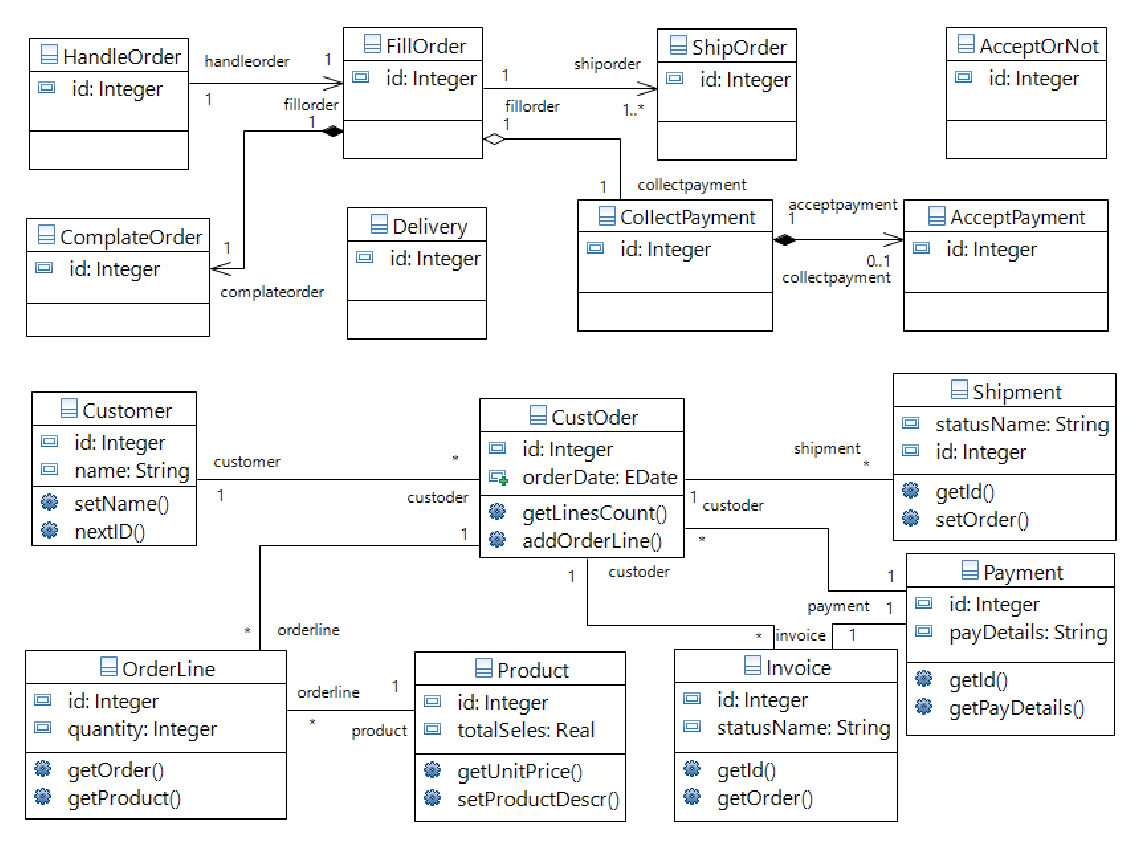
\includegraphics[scale=0.7]{domain-model-orderman}
\vspace{-0.5cm}
	\caption{the domain model of the \orderman} %
	\label{fig:domain-model-orderman}
	\vspace{-0.3cm}
\end{figure*}

To generate the unified domain model for \orderman, which is shown in Figure~\ref{fig:orderMan_unifiedModel}, we applied all the domain behavior patterns from our first catalog. Figure~\ref{fig:orderMan_unifiedModel}(A) presents an activity graph with nodes labeled with numbers that correspond to the activity HandleOrder. It also shows part of the unified class model, consisting of one activity class (HandleOrder), four primary data classes (\clazz{CustOrder}, \clazz{Invoice}, \clazz{Shipment}, \clazz{Payment}), four control classes (\clazz{AcceptOrNot}, \clazz{Delivery}, \clazz{CompleteOrder}, \clazz{EndOrder}), and four remaining classes related to coordinator nodes (\clazz{FillOrder}, \clazz{CollectPayment}, \clazz{ShipOrder}, \clazz{AcceptPayment}). As discussed in Section~\ref{sect:agl}, coordinator nodes are used to provide a complete view of a task group. For instance, the coordinator node FillOrder (node 3) manages two tasks, namely UpdateOrder (node 5) and DeliveryOrder (node 6). The FillOrder node simply coordinates the tasks to ensure that UpdateOrder is performed before DeliveryOrder. It does not contribute any data to the flow, but it enables the user to observe and execute the task flow on the UI.

\begin{figure*}[ht]
	\centering
	\includegraphics[scale=0.355]{orderMan_unifiedModel}
	\caption{(A: Left) The activity graph whose nodes are labeled with activity and component classes; (B: Top-right) The \clazz{Node} objects; (C: Bottom-right) \clazz{ModuleAct} objects that are referenced by the \clazz{Nodes}.} %
	\label{fig:orderMan_unifiedModel}
	\vspace{-0.2cm}
\end{figure*}

%Figure~\ref{fig:orderMan_unifiedModel}(B) highlights for each node of the activity graph (1)~the mapping from the node to a corresponding module (\wrt the domain class referenced by the \attribn{refCls}), (2)~the out nodes (\wrt the \attribn{refCls}), and (3)~the \clazz{ModuleAct} objects each of which specifies a SAA for the behavior of the module. These \clazz{ModuleAct} objects together with SAAs are listed in Figure~\ref{fig:orderMan_unifiedModel}(C). To obtain the \orderman software with the GUI, as shown in Figure~\ref{fig:orderManGUI}, %
%%GUIs like the one shown in Figure~\ref{fig:decisional-form-eg-gui}, 
%the unified class model incorporating the AGL specification (for the activity model) needs to be encoded in Java. The implemenation for \orderman is available at the git repository\footnote{\url{https://github.com/jdomainapp/orderman}}. Section~\ref{subsect:toolSupport} provides a detailed explanation of this implementation.
Figure~\ref{fig:orderMan_unifiedModel}(B) showcases how each node of the activity graph is mapped to a corresponding module (\wrt the domain class referenced by \attribn{refCls}), the out nodes (\wrt \attribn{refCls}), and the \clazz{ModuleAct} objects that specify SAAs for the module's behavior. These \clazz{ModuleAct} objects, along with SAAs, are listed in Figure~\ref{fig:orderMan_unifiedModel}(C). To develop the \orderman software with the GUI, as demonstrated in Figure~\ref{fig:orderManGUI}, the unified class model that integrates the \agl specification for the activity model must be encoded in Java. The implementation for \orderman can be found in the git repository\footnote{\url{https://github.com/jdomainapp/orderman}}. A detailed explanation of this implementation is presented in Section~\ref{subsect:toolSupport}.

\begin{figure*}[ht]
	\centering
	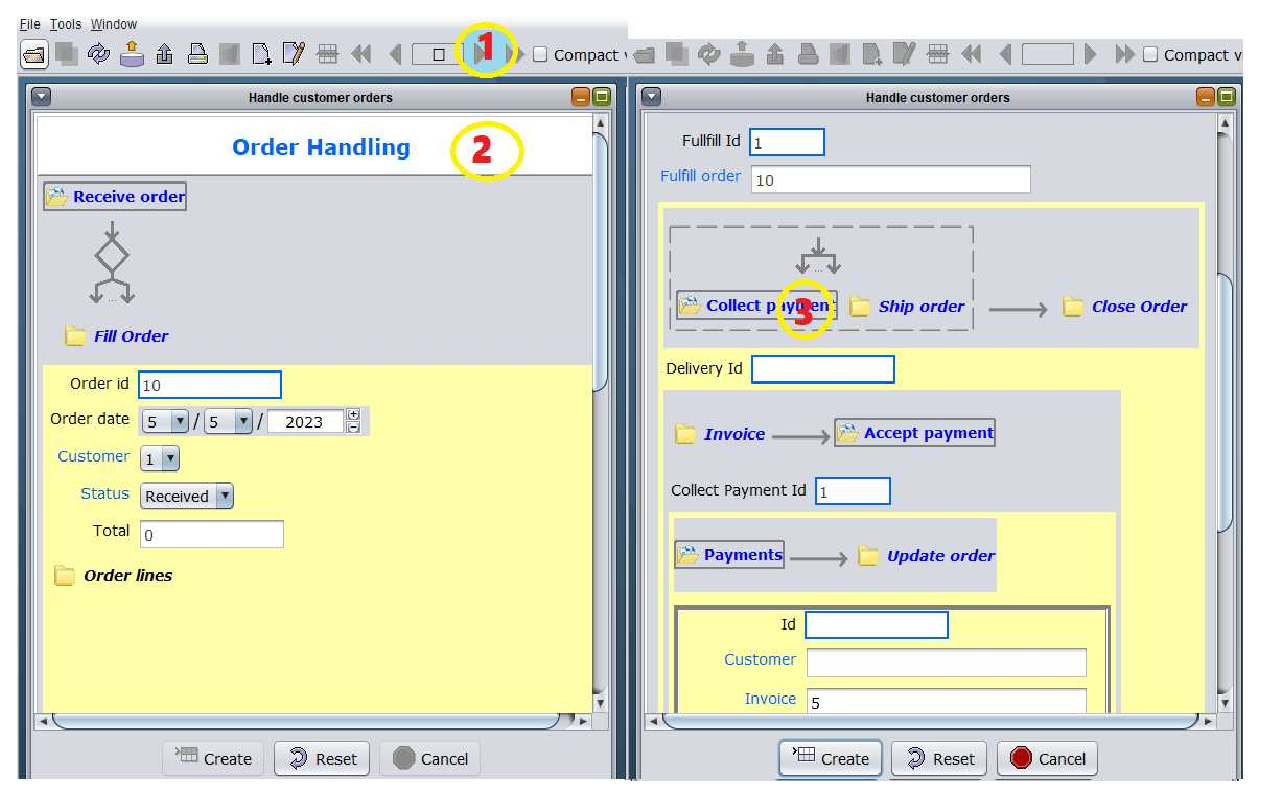
\includegraphics[scale=0.5]{orderManGUI}
	\caption{The GUI of the \orderman~software generated by the tool.} %
	\vspace{-0.3cm}
	\label{fig:orderManGUI}
\end{figure*}

%%%%%%%%%%%%%%%%%%%%%%%%%%%%%%%%%%%
\subsection{Tool Support}
\label{subsect:toolSupport} %
%%%%%%%%%%%%%%%%%%%%%%%%%%%%%%%%%%%%

%design choices and used technologies. For instance, this section could answer some of the following questions:
%- How annotations are inserted into Java or C code?
%- How the AGL is implemented?
%- What is the input format?

%As illustrated in Figure~\ref{fig:toolSupport}, we realized our method with a support tool based on JDomainApp, a Java software framework that we reported in previous works~\cite{le_domain_2018}. The tool is available at the git repository\footnote{\url{https://github.com/jdomainapp/jda-mbsl}}. %
The implementation of our method is demonstrated in Figure~\ref{fig:toolSupport}, using a supporting tool built on \jdomainapp, a Java software framework we have previously discussed in~\cite{le_domain_2018}. The tool can be accessed at the git repository\footnote{\url{https://github.com/jdomainapp/jda-mbsl}}.
%
%- What is the input format?
%To obtain a software generated from the input unified domain model, as explained in Section~\ref{sect:overviewApproach} and Definition~\ref{def:software}, the developer needs to encode the unified domain model in \dcsl and \agl, resulting in a Java program with two main parts: (1)~The \dcsl unified model, that consists of component and activity classes, as explained in Definition~\ref{def:unified-model}; (2)~The \agl specification for the activity graphs attached to the activity classes. Note that both the \dcsl and \agl specifications are encoded in Java, as illustrated in the middle and right windows (\resp) of Figure~\ref{fig:toolSupport}.
To generate software from the input unified domain model, as described in Section~\ref{sect:overviewApproach} and Definition~\ref{def:software}, the developer must encode the unified domain model in \dcsl and \agl, resulting in a Java program that has two main components: (1) The \dcsl unified model, which includes component and activity classes, as explained in Definition~\ref{def:unified-model}; (2) The \agl specification for the activity graphs associated with the activity classes. It is important to note that both the \dcsl and \agl specifications are encoded in Java, as depicted in the middle and right panels (\resp) of Figure~\ref{fig:toolSupport}.

\begin{figure*}[ht]
	\centering
	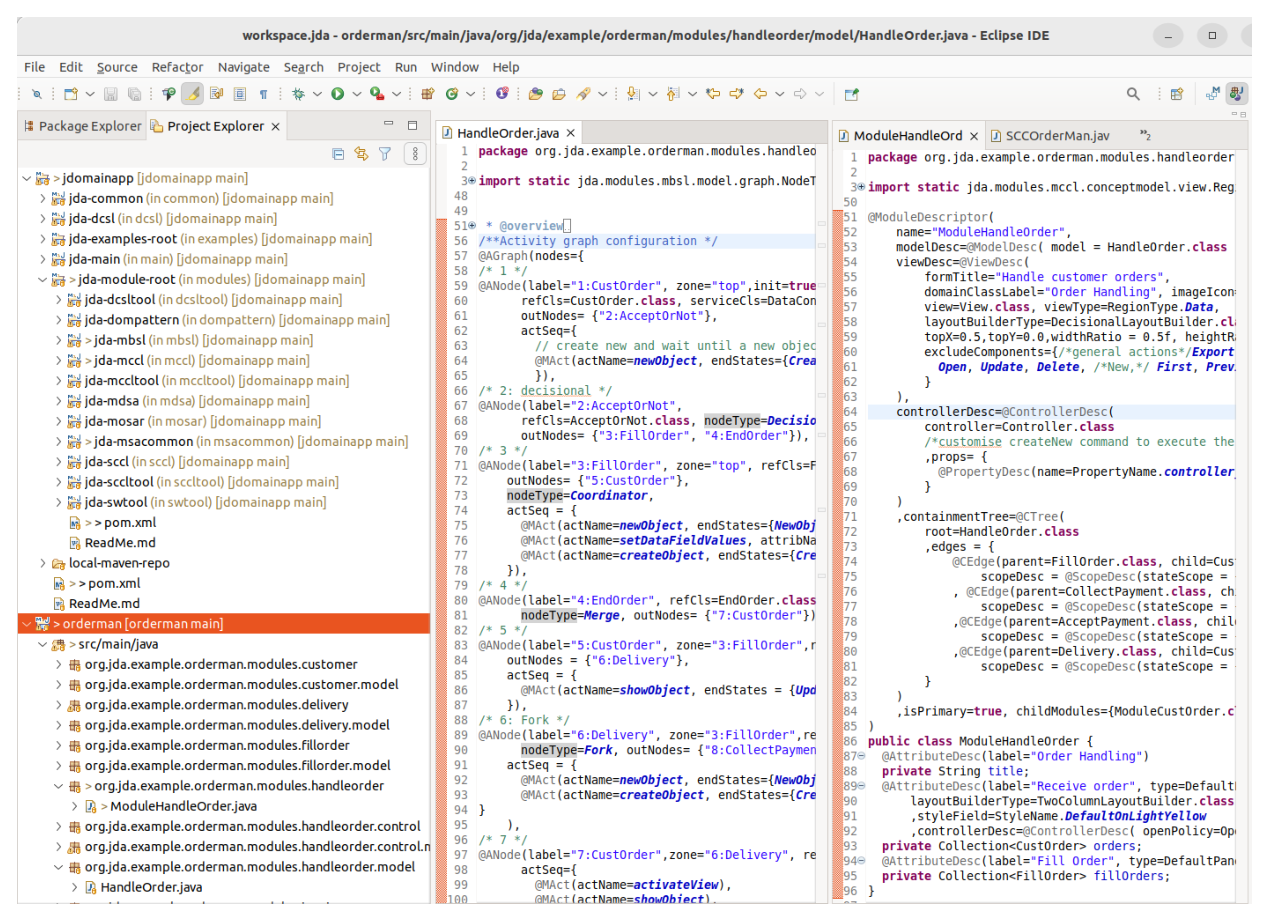
\includegraphics[scale=0.72]{toolSupport}
	\caption{Illustration for the JDomainApp-based realization and usability of \agl.} %
	\vspace{-0.2cm}
	\label{fig:toolSupport}
\end{figure*}

%Conceptually, the tool consists of three key components: model manager, view manager, and object manager. First, the \textbf{model manager} is responsible for registering the unified class model and making it accessible to other components. The left window in Figure~\ref{fig:toolSupport} depicts the list of module classes (e.g., \clazz{ModuleHandleOrder}) and corresponding domain classes (i.e., \clazz{HandleOrder}). As an activity domain class the \clazz{HandleOrder} is attached with an annotation \attribn{@AGraph} for the \agl specification, as presented in the middle window in Figure~\ref{fig:toolSupport}. The annotations to realize \agl are defined by the JDomainApp framework with the Java projects as shown in the left window of this figure. %
%Second, the \textbf{view manager} is responsible for (1) automatically generating the entire GUI of the software from the unified class model and (2) for handling the user interaction performed on this GUI. The GUI consists of a set of object UIs (one for each module's view), and a desktop for organizing these UIs. The two tasks basically are based on the configuration description of modules that is specified in MCCL~\cite{le_domain_2018}. For example, the module class \clazz{ModuleHandleOrder} that owns \clazz{HandleOrder}, as presented in the right window of this figure, is specified together with a module description in MCCL. %
%Third, the \textbf{object manager} is responsible for managing the run-time object pool of each domain class and for providing a generic object storage component for storing (retrieving) the objects to (from) external storage. As of this writing, the tool supports both file-based and relational database storage. The relational data model is automatically generated from the unified class model the first time the software is run.
The tool consists of three main components: the model manager, view manager, and object manager. The model manager registers and makes the unified class model available to other components. The left window of Figure~\ref{fig:toolSupport} displays a list of module classes and their corresponding domain classes that are attached with an annotation \attribn{@AGraph} for \agl specification, as presented in the middle window. The view manager automatically generates the GUI of the software and handles user interaction based on the configuration descriptions of modules specified in \mccl~\cite{le_domain_2018}. For instance, the module class \clazz{ModuleHandleOrder} that owns \clazz{HandleOrder} is specified with a module description in \mccl, as shown in the right window. Finally, the object manager manages the run-time object pool of each domain class and provides a generic object storage component that supports file-based and relational database storage. The relational data model is automatically generated from the unified class model when the software runs for the first time.

\vspace{0.1cm}
\noindent\begin{minipage}{.55\textwidth}
\begin{lstcodeplainssm}{The activity class \clazz{HandleOrder} in Java}{lst:handleOrderCls}
/**Activity graph configuration in AGL */
@AGraph(nodes={...	
	/* 14 */    
	@ANode(label="14:Payment", zone="11:AcceptPayment",
		refCls=Payment.class, serviceCls=DataController.class, 
		outNodes={"15:CustOrder"},
		actSeq={
			@MAct(actName=newObject, endStates={NewObject}),
			@MAct(actName=setDataFieldValues, attribNames={"invoice"},
				endStates={Created})
		}), ...
})
/**END: activity graph configuration */
public class HandleOrder {...}
\end{lstcodeplainssm}
\end{minipage}
\begin{minipage}{.45\textwidth}
%\vspace{-0.78cm}
\begin{lstcodeplainssm}{Java implementation of the annotation \attribn{AGraph}}{lst:aGraphAnnotation}
package jda.modules.mbsl.model.graph.meta;

import java.lang.annotation.*;
import jda.modules.mbsl.model.graph.ActivityGraph;

@Retention(RetentionPolicy.RUNTIME)
@Target(value=java.lang.annotation.ElementType.TYPE)
@Documented
public @interface AGraph {
	ANode[] nodes();
}
\end{lstcodeplainssm}	
\end{minipage}
%\vspace{0.2cm}

%We would further explain how a module class \wrt an activity class can handle the execution of the activity graph \wrt its AGL specification. Let's focus on a concrete situation with the  \clazz{ModuleHandleOrder} module \wrt the activity class \clazz{HandleOrder}, realized as in Listing~\ref{lst:handleOrderCls}. %
%%
%When the software runs, an instance of the \clazz{ModuleHandleOrder} module is invoked. Based on the configuration description of this module as shown in the right window of Figure~\ref{fig:toolSupport}, an activity model (\clazz{ActivityModel}) as a composition of the \clazz{HandleOrder} object \wrt the \clazz{ModuleHandleOrder} module and the activity graph \wrt the AGL specification of the activity class \clazz{HandleOrder} is created. Based on the annotation mechanism in Java, the \clazz{HandleOrder} object can be viewed as an \clazz{AGraph} object, and then this \clazz{AGraph} object could represent and handle the activity graph: The \clazz{AGraph} object allows each of its \clazz{ANode}, e.g., the \clazz{ANode} \wrt node~14 as shown in Listing~\ref{lst:handleOrderCls}, as well as the domain class referenced by the \clazz{ANode} (i.e., the \clazz{Payment} class) could be handled by the \clazz{ModuleHandleOrder} module. For a detailed implementation of this activity model, we would refer the reader to Appendix C of the accompanying technical report~\cite{dang2023aglTechReport}.
We will further clarify how a module class (\wrt an activity class) can manage the execution of the activity graph (\wrt the activity class) based on its \agl specification. Let's consider a specific scenario with the \clazz{ModuleHandleOrder} module and the \clazz{HandleOrder} activity class, implemented as shown in Listing~\ref{lst:handleOrderCls}. When the software runs, an instance of the \clazz{ModuleHandleOrder} module is called. Using the module's configuration description presented in the right window of Figure~\ref{fig:toolSupport}, an \clazz{ActivityModel} is created as a composition of the \clazz{HandleOrder} object \wrt the \clazz{ModuleHandleOrder} module and the activity graph specified by the \agl for the \clazz{HandleOrder} activity class. %
%
Using the annotation mechanism in Java, the \clazz{HandleOrder} object can be treated as an \clazz{AGraph} object, allowing it to represent and manage the activity graph. The \clazz{AGraph} object enables the \clazz{ModuleHandleOrder} module to handle each of its \clazz{ANode}s, such as the \clazz{ANode} \wrt node 14 in Listing~\ref{lst:handleOrderCls}, as well as the domain class referred to by the \clazz{ANode}, in this case, the \clazz{Payment} class. For a more detailed implementation of this activity model is presented in Appendix~C.

%- How annotations are inserted into Java or C code?
%- How the AGL is implemented?
We will further explain how the \agl and its annotations is realized in Java. The \agl specification of an activity class is represented as an annotation of the activity class in Java. For example, Listing~\ref{lst:handleOrderCls} illustrates the annotation used to express the \agl specification of the \clazz{HandleOrder} activity class. All the annotations in \agl, as summarized in Figure~\ref{fig:agl-txtSyntax}, have to be defined in Java. Listing~\ref{lst:aGraphAnnotation} provides an example of such a definition for the \clazz{AGraph} annotation, and the other annotations in \agl are defined similarly.